\documentclass{article}
\usepackage{amsmath}
\usepackage{amsfonts}
\usepackage{mathtools}
\usepackage{tikz}
\usetikzlibrary{calc}
\usepackage[utf8]{inputenc}
\usetikzlibrary {arrows.meta, angles, quotes}

\begin{document}

\section*{Bevezetés}
Kezdjük néhány nagyon egyszerű dologgal. Először is tekintsünk egy téglalapot.
\begin{center}
\centering
\begin{tikzpicture}[>=Stealth]
    \coordinate (O) at ( 0.0, 0.0);
    \coordinate (A) at ( 3.0, 0.0);
    \coordinate (B) at ( 3.0, 1.5);
    \coordinate (C) at ( 0.0, 1.5);
    \draw (O) -- (A) -- (B) -- (C) -- cycle;
    % b betű bal oldalon középen (a C-O élen)
    \node[left] at ($(C)!0.5!(O)$) {$b$};

    % a betű alul középen (az O-A élen)
    \node[below] at ($(O)!0.5!(A)$) {$a$};

    % Terület jobbra mellette (a B és A pont felezőpontjának magasságában)
    \node[right] at (3.6, 0.75) {$A = a \cdot b$};
\end{tikzpicture}
\end{center}
A téglalap mellett látható a terület nagysága. Itt a nagy $A$ betű a területet jelenti (Area). A területet tehát a hosszúság szorozva a magassággal képlettel számítjuk ki.

Ha most húzunk egy átlót bal fentről jobb lefelé, a téglalapot két egyenlő részre osztjuk. Ha az egyik háromszöget zöld színnel kitöltjük, a következőt érjük el:
\begin{center}
\centering
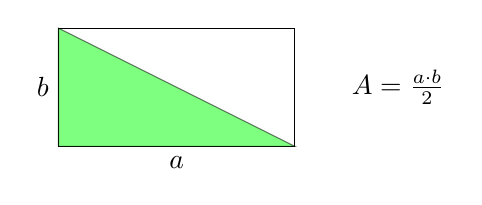
\begin{tikzpicture}[>=Stealth]
    \coordinate (O) at ( 0.0, 0.0);
    \coordinate (A) at ( 3.0, 0.0);
    \coordinate (B) at ( 3.0, 1.5);
    \coordinate (C) at ( 0.0, 1.5);
    \draw (O) -- (A) -- (B) -- (C) -- cycle;

    % b betű bal oldalon középen (a C-O élen)
    \node[left] at ($(C)!0.5!(O)$) {$b$};

    % a betű alul középen (az O-A élen)
    \node[below] at ($(O)!0.5!(A)$) {$a$};

    % Terület jobbra mellette (a B és A pont felezőpontjának magasságában)
    \node[right] at (3.6, 0.75) {$A = \frac{a \cdot b}{2}$};
    % Átló kitöltött háromszöggel
    \draw [draw=black, fill=green, opacity=0.5]
    (O) -- (A) -- (C) -- cycle;
\end{tikzpicture}
\end{center}
Ebből látható, hogy a háromszög területe a fele a téglalap területének.
Most rajzoljunk egy másik háromszöget a téglalapba.
\begin{center}
\centering
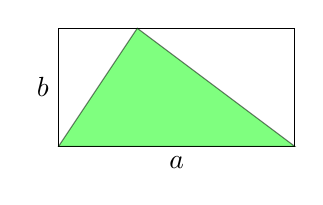
\begin{tikzpicture}[>=Stealth]
    \coordinate (O) at ( 0.0, 0.0);
    \coordinate (A) at ( 3.0, 0.0);
    \coordinate (B) at ( 3.0, 1.5);
    \coordinate (C) at ( 0.0, 1.5);
    \draw (O) -- (A) -- (B) -- (C) -- cycle;

    % b betű bal oldalon középen (a C-O élen)
    \node[left] at ($(C)!0.5!(O)$) {$b$};

    % a betű alul középen (az O-A élen)
    \node[below] at ($(O)!0.5!(A)$) {$a$};

    % Átló kitöltött háromszöggel
    \coordinate (C) at ( 1.0, 1.5);
    \draw [draw=black, fill=green, opacity=0.5]
    (O) -- (A) -- (C) -- cycle;

\end{tikzpicture}
\end{center}
Hogyan lehetne kiszámítani ennek a háromszögnek a területét? Az egyik ötlet az, hogy a háromszög csúcsából állítunk egy merőlegest, hogy így a háromszöget két részre bontsuk.

\section{A háromszög területének levezetése}

Egy általános háromszög területének kiszámításához a háromszöget egy \textbf{merőleges} (a $h$ magasság) segítségével két derékszögű rész-háromszögre bonthatjuk.

\begin{center}
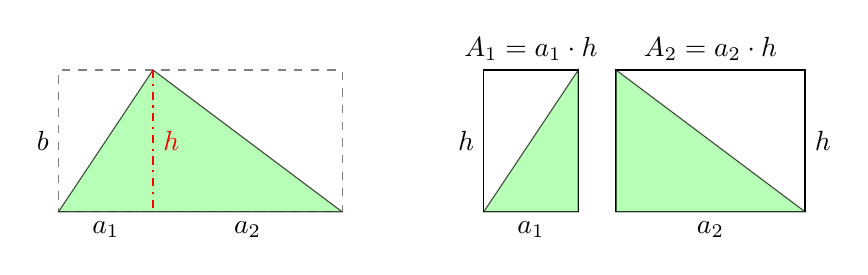
\begin{tikzpicture}[>=Stealth, scale=1.2]

    % --- BAL OLDALI KÉP: Téglalap a háromszögben lévő merőlegessel ---
    \coordinate (O) at (0.0, 0.0);
    \coordinate (A) at (3.0, 0.0);
    \coordinate (B) at (3.0, 1.5);
    \coordinate (TopL) at (0.0, 1.5);
    \coordinate (C) at (1.0, 1.5); % A háromszög csúcsa
    \coordinate (H) at (1.0, 0.0); % A merőleges talppontja

    % Téglalap külső kerete
    \draw[dashed, gray] (O) -- (A) -- (B) -- (TopL) -- cycle;

    % Zöld háromszög
    \draw [draw=black, fill=green!40, opacity=0.7] (O) -- (A) -- (C) -- cycle;

    % Merőleges (h magasság) berajzolása
    \draw[red, thick, dash dot] (C) -- (H) node[midway, right] {$h$};

    % Az alapszakaszok feliratai
    \node[below] at ($(O)!0.5!(H)$) {$a_1$};
    \node[below] at ($(H)!0.5!(A)$) {$a_2$};
    \node[left] at ($(TopL)!0.5!(O)$) {$b$};

    % --- JOBB OLDALI KÉP: Különálló rész-téglalapok ---
    % Eltolás jobbra: Shift-X 4.5 cm-rel
    \begin{scope}[xshift=4.5cm]

        % 1. rész-téglalap (balra, szélessége a1 = 1.0)
        \coordinate (O1) at (0.0, 0.0);
        \coordinate (A1) at (1.0, 0.0);
        \coordinate (B1) at (1.0, 1.5);
        \coordinate (C1) at (0.0, 1.5);

        \draw (O1) -- (A1) -- (B1) -- (C1) -- cycle;
        \draw[fill=green!40, opacity=0.7] (O1) -- (A1) -- (B1) -- cycle;

        \node[below] at (0.5, 0) {$a_1$};
        \node[left] at (0, 0.75) {$h$};
        \node[above] at (0.5, 1.5) {$A_1 = a_1 \cdot h$};

        % 2. rész-téglalap (jobbra, enyhén elkülönítve 0.4 cm távolságra, szélessége a2 = 2.0)
        \begin{scope}[xshift=1.4cm]
            \coordinate (O2) at (0.0, 0.0);
            \coordinate (A2) at (2.0, 0.0);
            \coordinate (B2) at (2.0, 1.5);
            \coordinate (C2) at (0.0, 1.5);

            \draw (O2) -- (A2) -- (B2) -- (C2) -- cycle;
            \draw[fill=green!40, opacity=0.7] (O2) -- (A2) -- (C2) -- cycle;

            \node[below] at (1.0, 0) {$a_2$};
            \node[right] at (2.0, 0.75) {$h$};
            \node[above] at (1.0, 1.5) {$A_2 = a_2 \cdot h$};
        \end{scope}
    \end{scope}

\end{tikzpicture}
\end{center}
\begin{enumerate}
    \item \textbf{Az alap felbontása:} A csúcsból az $a$ alapra bocsátott merőleges azt két $a_1$ és $a_2$ szakaszra osztja, így érvényes:
    $$a = a_1 + a_2$$

    \item \textbf{A rész-téglalapok vizsgálata:} Mindkét rész-háromszög beágyazható egy-egy saját téglalapba:
    \begin{itemize}
        \item A bal oldali rész-háromszög területe a bal oldali rész-téglalap területének a fele:
        $$A_1 = \frac{1}{2} \cdot a_1 \cdot h$$
        \item A jobb oldali rész-háromszög területe a jobb oldali rész-téglalap területének a fele:
        $$A_2 = \frac{1}{2} \cdot a_2 \cdot h$$
    \end{itemize}

    \item \textbf{A teljes terület összeállítása:} A háromszög teljes $A$ területe a két rész-háromszög összegéből adódik:
    $$A = A_1 + A_2 = \frac{1}{2} \cdot a_1 \cdot h + \frac{1}{2} \cdot a_2 \cdot h$$

    Az $\frac{1}{2} \cdot h$ kiemelésével kapjuk a jól ismert képletet:
    $$A = \frac{1}{2} \cdot (a_1 + a_2) \cdot h \implies A = \frac{1}{2} \cdot a \cdot h$$
\end{enumerate}

Íme egy vizuális szemléltetés arról, hogy minden azonos $a$ hosszúságú és azonos $h$ magasságú háromszög területe azonos.

\begin{center}
\centering
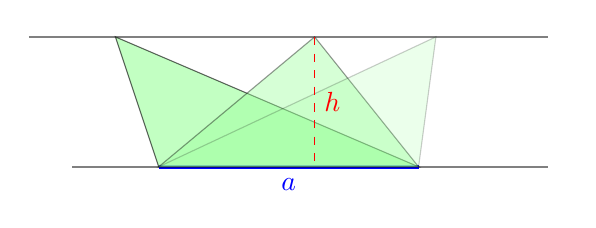
\begin{tikzpicture}[>=Stealth, scale=1.1]
    % Párhuzamos egyenesek (a rudak)
    \draw[thick, gray] (-1.0, 0.0) -- (4.5, 0.0) node[right] {};
    \draw[thick, gray] (-1.5, 1.5) -- (4.5, 1.5) node[right] {};

    % a alap (rögzített rúd)
    \coordinate (O) at (0.0, 0.0);
    \coordinate (A) at (3.0, 0.0);
    \draw[ultra thick, blue] (O) -- (A) node[midway, below] {$a$};

    % Első háromszög (balra eltolt csúcs)
    \coordinate (B1) at (-0.5, 1.5);
    \draw [draw=black, fill=green!40, opacity=0.6] (O) -- (A) -- (B1) -- cycle;

    % Második háromszög (csúcs középen)
    \coordinate (B2) at (1.8, 1.5);
    \draw [draw=black, fill=green!40, opacity=0.4] (O) -- (A) -- (B2) -- cycle;

    % Harmadik háromszög (jobbra eltolt csúcs)
    \coordinate (B3) at (3.2, 1.5);
    \draw [draw=black, fill=green!40, opacity=0.2] (O) -- (A) -- (B3) -- cycle;

    % Szaggatott h magasság demonstrációként
    \draw[red, dashed] (1.8, 1.5) -- (1.8, 0.0) node[midway, right] {$h$};

\end{tikzpicture}
\end{center}

Elképzelheted úgy, hogy a háromszög alsó oldala egy rögzített rúd, a háromszög csúcsa pedig egy másik rúdon mozgatható, két gumiszalaggal összekötve. Ha a csúcsot elmozgatod a felső rúd mentén, a háromszög területe mindig ugyanaz marad.

\end{document}
